\documentclass[12pt,a4paper]{article}

% Packages
\usepackage[utf8]{inputenc}
\usepackage[T1]{fontenc}
\usepackage{geometry}
\usepackage{graphicx}
\usepackage{hyperref}
\usepackage{enumitem}
\usepackage{xcolor}
\usepackage{tikz}
\usepackage{booktabs}
\usepackage{fancyhdr}
\usepackage{tcolorbox}
\usepackage{listings}
\usepackage{amsmath}
\usepackage{amssymb}

% Page geometry
\geometry{margin=2.5cm}

% Colors
\definecolor{primaryblue}{RGB}{0, 102, 204}
\definecolor{successgreen}{RGB}{40, 167, 69}
\definecolor{dangerred}{RGB}{220, 53, 69}
\definecolor{warningyellow}{RGB}{255, 193, 7}
\definecolor{lightgray}{RGB}{248, 249, 250}
\definecolor{codegray}{RGB}{45, 45, 45}
\definecolor{codegreen}{RGB}{0, 128, 0}

% TikZ libraries
\usetikzlibrary{shapes, arrows, positioning, fit, backgrounds, calc}

% Listings setup for code
\lstset{
    basicstyle=\ttfamily\small,
    backgroundcolor=\color{lightgray},
    frame=single,
    framerule=0pt,
    breaklines=true,
    showstringspaces=false,
    keywordstyle=\color{primaryblue}\bfseries,
    commentstyle=\color{codegreen},
    stringstyle=\color{dangerred},
    numbers=left,
    numberstyle=\tiny\color{gray},
    numbersep=5pt,
    xleftmargin=15pt
}

% Header and footer
\pagestyle{fancy}
\fancyhf{}
\fancyhead[L]{\textbf{CS2113 -- Software Development Project}}
\fancyhead[R]{Lecture 2: Git \& GitHub}
\fancyfoot[C]{\thepage}

% Tcolorbox styles
\tcbuselibrary{skins, breakable, listings}

\newtcolorbox{keyinsight}{
    colback=primaryblue!10,
    colframe=primaryblue,
    title=\textbf{Key Insight},
    fonttitle=\bfseries,
    breakable
}

\newtcolorbox{warning}{
    colback=dangerred!10,
    colframe=dangerred,
    title=\textbf{Warning},
    fonttitle=\bfseries,
    breakable
}

\newtcolorbox{tip}{
    colback=successgreen!10,
    colframe=successgreen,
    title=\textbf{Tip},
    fonttitle=\bfseries,
    breakable
}

\newtcolorbox{commandbox}{
    colback=codegray!10,
    colframe=codegray,
    fonttitle=\bfseries,
    breakable
}

\newtcolorbox{definitionbox}{
    colback=lightgray,
    colframe=black!50,
    breakable
}

% Title
\title{
    \vspace{-1cm}
    \textbf{Version Control: Git and GitHub}\\
    \large Lecture 2 Notes\\[0.5cm]
    \normalsize School of Computing Communication and Media Studies
}
\author{Masoud Hamad}
\date{CS2113 -- Software Development Project\\Academic Year 2025}

\begin{document}

\maketitle
\tableofcontents
\newpage

%============================================================
\section{Introduction to Version Control}
%============================================================

\begin{definitionbox}
\textbf{Version Control} is a system for storing code that enables:
\begin{itemize}
    \item Storing backups of current and older program versions
    \item Enabling code/project sharing for collaboration
    \item Marking specific project states for recovery
    \item Tracking developer contributions and changes
    \item Facilitating bug identification
\end{itemize}
\end{definitionbox}

\begin{keyinsight}
Version control enables ``using and developing others' code, even without ever meeting in person.'' It is one of the most vital skills required in professional software development.
\end{keyinsight}

%------------------------------------------------------------
% Figure 1: Version Control Benefits
%------------------------------------------------------------
\begin{figure}[htbp]
\centering
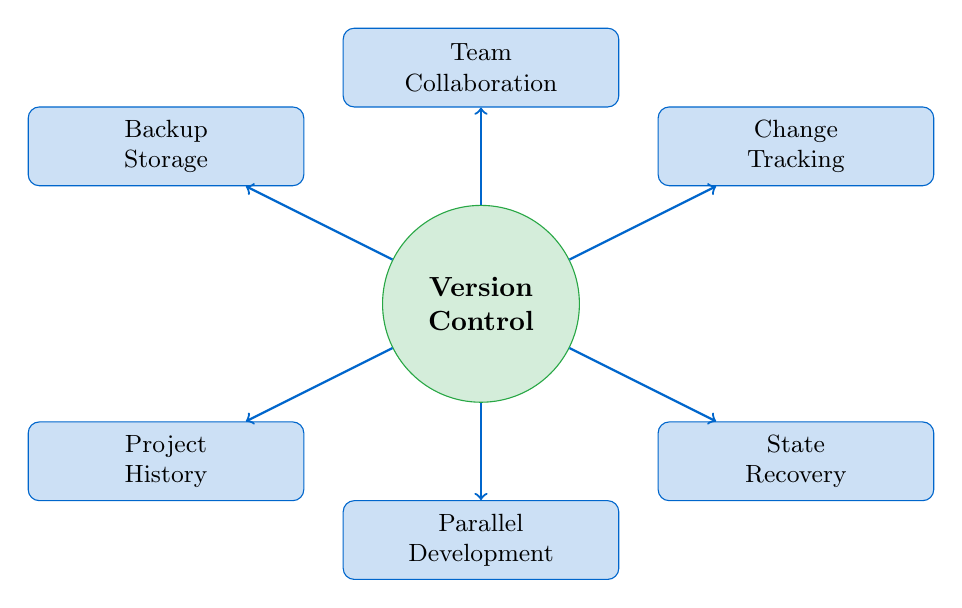
\begin{tikzpicture}[
    node distance=1cm,
    benefit/.style={rectangle, draw=primaryblue, fill=primaryblue!20, rounded corners, minimum width=3.5cm, minimum height=1cm, align=center, font=\small},
    center/.style={circle, draw=successgreen, fill=successgreen!20, minimum size=2.5cm, align=center, font=\bfseries}
]
    \node[center] (vc) at (0,0) {Version\\Control};

    \node[benefit] (backup) at (-4, 2) {Backup\\Storage};
    \node[benefit] (collab) at (0, 3) {Team\\Collaboration};
    \node[benefit] (track) at (4, 2) {Change\\Tracking};
    \node[benefit] (history) at (-4, -2) {Project\\History};
    \node[benefit] (branch) at (0, -3) {Parallel\\Development};
    \node[benefit] (recover) at (4, -2) {State\\Recovery};

    \draw[->, thick, primaryblue] (vc) -- (backup);
    \draw[->, thick, primaryblue] (vc) -- (collab);
    \draw[->, thick, primaryblue] (vc) -- (track);
    \draw[->, thick, primaryblue] (vc) -- (history);
    \draw[->, thick, primaryblue] (vc) -- (branch);
    \draw[->, thick, primaryblue] (vc) -- (recover);
\end{tikzpicture}
\caption{Benefits of Version Control Systems}
\label{fig:vc-benefits}
\end{figure}

%============================================================
\section{About Git}
%============================================================

\subsection{History and Origin}

\textbf{Git} was created by \textbf{Linus Torvalds}, the developer of the Linux kernel. Torvalds created it to manage Linux kernel code versions and share them with collaborators.

\subsection{Related Platforms}

\begin{itemize}
    \item \textbf{GitHub:} Service for storing and publishing projects (most popular)
    \item \textbf{GitLab:} Similar alternative platform with CI/CD features
    \item \textbf{Bitbucket:} Atlassian's Git hosting service
\end{itemize}

\begin{tip}
Git and GitHub are used in solo and collaborative projects across the industry. Applications extend beyond code---many people backup their course materials, documentation, and other files using Git.
\end{tip}

%============================================================
\section{Installation and Setup}
%============================================================

\subsection{Installing Git}

\begin{itemize}
    \item \textbf{Windows:} Download Git for Windows from \texttt{gitforwindows.org}
    \item \textbf{macOS:} Install via Homebrew: \texttt{brew install git}
    \item \textbf{Linux:} Use package manager: \texttt{sudo apt install git}
\end{itemize}

\subsection{Initial Configuration}

After installation, configure Git with your identity:

\begin{commandbox}
\begin{lstlisting}[language=bash]
git config --global user.name "Your Name"
git config --global user.email "your.email@example.com"
git config --global init.defaultBranch main
\end{lstlisting}
\end{commandbox}

\begin{warning}
Use the same email address as your GitHub account. If you don't want your email to be public, GitHub offers a specific noreply email address.
\end{warning}

%============================================================
\section{Git Fundamentals}
%============================================================

\subsection{Starting a Git Project}

A project is simply a folder containing files. Initialize with:

\begin{commandbox}
\begin{lstlisting}[language=bash]
git init
\end{lstlisting}
\end{commandbox}

This creates a \texttt{.git} subfolder storing all project metadata and history.

\subsection{Understanding Commits}

\begin{definitionbox}
A \textbf{commit} is a bundle of changes made to files inside the project. In practice, these changes are often adding or removing text from files.
\end{definitionbox}

Commits function as ``steps towards a finished project.'' Every commit adds some changes to the previous commit.

%------------------------------------------------------------
% Figure 2: Commit History
%------------------------------------------------------------
\begin{figure}[htbp]
\centering
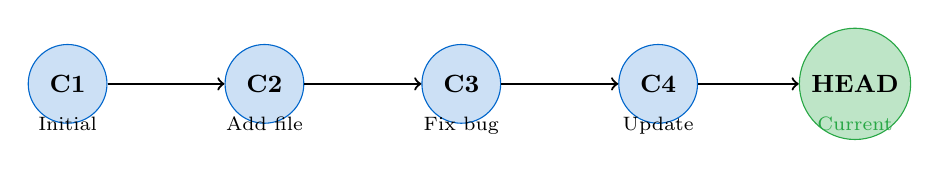
\begin{tikzpicture}[
    node distance=2cm,
    commit/.style={circle, draw=primaryblue, fill=primaryblue!20, minimum size=1cm, font=\small\bfseries},
    arrow/.style={->, thick}
]
    \node[commit] (c1) at (0, 0) {C1};
    \node[commit] (c2) at (2.5, 0) {C2};
    \node[commit] (c3) at (5, 0) {C3};
    \node[commit] (c4) at (7.5, 0) {C4};
    \node[commit, fill=successgreen!30, draw=successgreen] (head) at (10, 0) {HEAD};

    \draw[arrow] (c1) -- (c2);
    \draw[arrow] (c2) -- (c3);
    \draw[arrow] (c3) -- (c4);
    \draw[arrow] (c4) -- (head);

    \node[below=0.3cm, font=\scriptsize] at (c1) {Initial};
    \node[below=0.3cm, font=\scriptsize] at (c2) {Add file};
    \node[below=0.3cm, font=\scriptsize] at (c3) {Fix bug};
    \node[below=0.3cm, font=\scriptsize] at (c4) {Update};
    \node[below=0.3cm, font=\scriptsize, successgreen] at (head) {Current};
\end{tikzpicture}
\caption{Git Commit History as a Linear Chain}
\label{fig:commit-history}
\end{figure}

\subsection{The Commit Process}

\begin{enumerate}
    \item Make changes to files
    \item \textbf{Stage} changes using \texttt{git add}
    \item \textbf{Create commit} using \texttt{git commit}
    \item Check status with \texttt{git status}
\end{enumerate}

%============================================================
\section{File States in Git}
%============================================================

The \texttt{git status} command reveals three possible states:

%------------------------------------------------------------
% Figure 3: Git File States
%------------------------------------------------------------
\begin{figure}[htbp]
\centering
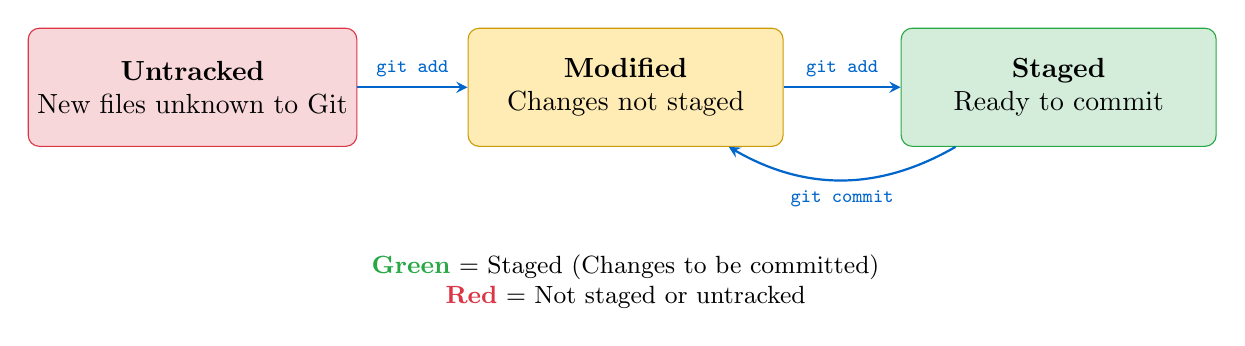
\begin{tikzpicture}[
    node distance=1.5cm,
    state/.style={rectangle, draw, rounded corners, minimum width=4cm, minimum height=1.5cm, align=center},
    arrow/.style={->, thick, >=stealth}
]
    \node[state, fill=dangerred!20, draw=dangerred] (untracked) at (0, 0) {\textbf{Untracked}\\New files unknown to Git};
    \node[state, fill=warningyellow!30, draw=warningyellow!80!black] (modified) at (5.5, 0) {\textbf{Modified}\\Changes not staged};
    \node[state, fill=successgreen!20, draw=successgreen] (staged) at (11, 0) {\textbf{Staged}\\Ready to commit};

    \draw[arrow, primaryblue] (untracked) -- node[above, font=\scriptsize] {\texttt{git add}} (modified);
    \draw[arrow, primaryblue] (modified) -- node[above, font=\scriptsize] {\texttt{git add}} (staged);
    \draw[arrow, primaryblue, bend left=30] (staged) to node[below, font=\scriptsize] {\texttt{git commit}} (modified);

    \node[below=2cm, align=center, font=\small] at (5.5, 0) {
        \textcolor{successgreen}{\textbf{Green}} = Staged (Changes to be committed)\\
        \textcolor{dangerred}{\textbf{Red}} = Not staged or untracked
    };
\end{tikzpicture}
\caption{Git File States and Transitions}
\label{fig:file-states}
\end{figure}

\subsection{State Descriptions}

\begin{enumerate}
    \item \textbf{Changes to be committed (Staging Area):}
    \begin{itemize}
        \item Changes ready for the next commit
        \item Displayed in \textcolor{successgreen}{green}
        \item Add files via \texttt{git add}
        \item Remove via \texttt{git rm --cached}
    \end{itemize}

    \item \textbf{Changes not staged for commit:}
    \begin{itemize}
        \item Modified tracked files not yet staged
        \item Undo via \texttt{git restore filename}
    \end{itemize}

    \item \textbf{Untracked files:}
    \begin{itemize}
        \item New files unknown to Git
        \item Must be added with \texttt{git add}
    \end{itemize}
\end{enumerate}

\begin{keyinsight}
Git tracks \textit{changes}. When you create a file, the ``change'' is the file creation. When you modify it, the ``change'' is the modification. Each change must be staged before committing.
\end{keyinsight}

%============================================================
\section{Essential Git Commands}
%============================================================

\subsection{Adding Changes}

\begin{commandbox}
\begin{lstlisting}[language=bash]
# Add a single file
git add filename.txt

# Add all files in a folder
git add folder_name/

# Add all changes in the project
git add .

# Interactive selection (tracked files only)
git add -p
\end{lstlisting}
\end{commandbox}

\subsection{Creating Commits}

\begin{commandbox}
\begin{lstlisting}[language=bash]
# Quick commit with message
git commit -m "Descriptive commit message"

# Open editor for detailed message
git commit
\end{lstlisting}
\end{commandbox}

\begin{tip}
Write clear, descriptive commit messages that explain \textit{why} the change was made, not just \textit{what} changed.
\end{tip}

\subsection{Viewing History}

\begin{commandbox}
\begin{lstlisting}[language=bash]
# View commit history
git log

# Compact one-line format
git log --oneline

# View changes in a specific commit
git show commit_id
\end{lstlisting}
\end{commandbox}

%============================================================
\section{Branches}
%============================================================

\begin{definitionbox}
\textbf{Branches} allow separating commits from each other. A new branch can be developed independently from the main branch without affecting it.
\end{definitionbox}

\subsection{Branch Terminology}

\begin{itemize}
    \item \textbf{main} (modern standard): The primary branch
    \item \textbf{master} (traditional): Legacy name for primary branch
    \item \textbf{HEAD}: Points to the current commit/branch
\end{itemize}

%------------------------------------------------------------
% Figure 4: Git Branching
%------------------------------------------------------------
\begin{figure}[htbp]
\centering
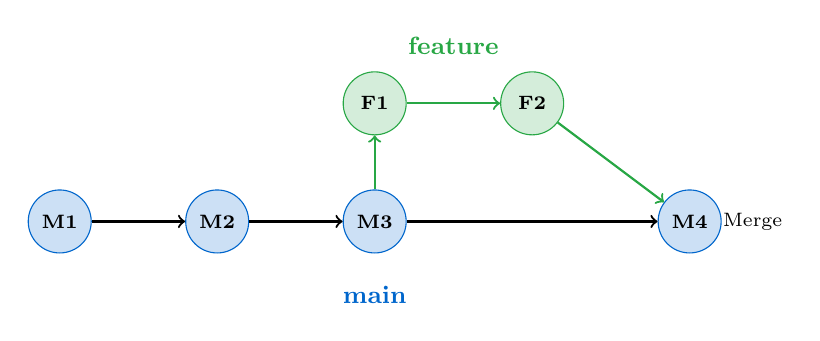
\begin{tikzpicture}[
    node distance=1.5cm,
    commit/.style={circle, draw=primaryblue, fill=primaryblue!20, minimum size=0.8cm, font=\scriptsize\bfseries},
    feature/.style={circle, draw=successgreen, fill=successgreen!20, minimum size=0.8cm, font=\scriptsize\bfseries},
    arrow/.style={->, thick}
]
    % Main branch
    \node[commit] (m1) at (0, 0) {M1};
    \node[commit] (m2) at (2, 0) {M2};
    \node[commit] (m3) at (4, 0) {M3};
    \node[commit] (m4) at (8, 0) {M4};

    % Feature branch
    \node[feature] (f1) at (4, 1.5) {F1};
    \node[feature] (f2) at (6, 1.5) {F2};

    % Arrows
    \draw[arrow] (m1) -- (m2);
    \draw[arrow] (m2) -- (m3);
    \draw[arrow, successgreen] (m3) -- (f1);
    \draw[arrow, successgreen] (f1) -- (f2);
    \draw[arrow, successgreen] (f2) -- (m4);
    \draw[arrow] (m3) -- (m4);

    % Labels
    \node[below=0.2cm, primaryblue, font=\small\bfseries] at (4, -0.5) {main};
    \node[above=0.2cm, successgreen, font=\small\bfseries] at (5, 1.8) {feature};

    % Merge point
    \node[right=0.3cm, font=\scriptsize] at (m4) {Merge};
\end{tikzpicture}
\caption{Git Branching and Merging}
\label{fig:branching}
\end{figure}

\subsection{Branch Commands}

\begin{commandbox}
\begin{lstlisting}[language=bash]
# Create a new branch
git branch feature-name

# Switch to a branch
git checkout feature-name

# Create and switch in one command
git checkout -b feature-name

# List all branches
git branch

# Delete a branch
git branch -d feature-name
\end{lstlisting}
\end{commandbox}

%============================================================
\section{Working with GitHub (Remote Repositories)}
%============================================================

\subsection{Remote Repository Concept}

\begin{definitionbox}
A \textbf{remote repository} is a version of your project hosted on a server (like GitHub). It enables sharing code with others and serves as a backup.
\end{definitionbox}

%------------------------------------------------------------
% Figure 5: Local vs Remote Repository
%------------------------------------------------------------
\begin{figure}[htbp]
\centering
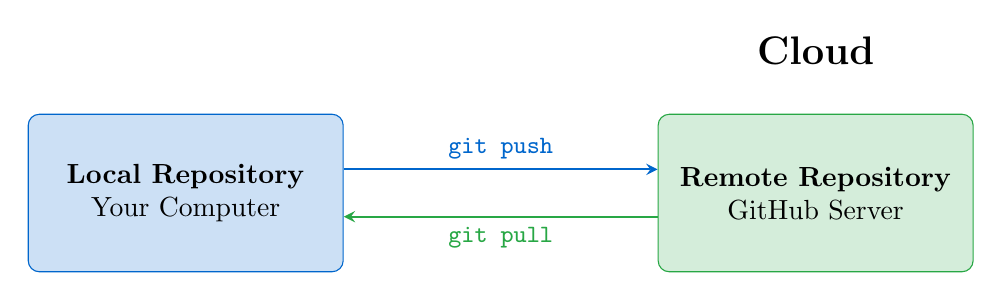
\begin{tikzpicture}[
    node distance=2cm,
    repo/.style={rectangle, draw, rounded corners, minimum width=4cm, minimum height=2cm, align=center},
    arrow/.style={->, thick, >=stealth}
]
    \node[repo, fill=primaryblue!20, draw=primaryblue] (local) at (0, 0) {\textbf{Local Repository}\\Your Computer};
    \node[repo, fill=successgreen!20, draw=successgreen] (remote) at (8, 0) {\textbf{Remote Repository}\\GitHub Server};

    \draw[arrow, primaryblue] ([yshift=0.3cm]local.east) -- node[above, font=\small] {\texttt{git push}} ([yshift=0.3cm]remote.west);
    \draw[arrow, successgreen] ([yshift=-0.3cm]remote.west) -- node[below, font=\small] {\texttt{git pull}} ([yshift=-0.3cm]local.east);

    % Cloud icon
    \node[above=0.5cm] at (remote.north) {\Large\textbf{Cloud}};
\end{tikzpicture}
\caption{Synchronization Between Local and Remote Repositories}
\label{fig:local-remote}
\end{figure}

\subsection{Adding a Remote}

\begin{commandbox}
\begin{lstlisting}[language=bash]
# Add a remote repository
git remote add origin https://github.com/username/repo.git

# View configured remotes
git remote -v
\end{lstlisting}
\end{commandbox}

\subsection{Push and Pull}

\begin{commandbox}
\begin{lstlisting}[language=bash]
# Push changes to remote (first time)
git push -u origin main

# Push subsequent changes
git push

# Pull changes from remote
git pull

# Fetch without merging
git fetch
\end{lstlisting}
\end{commandbox}

\begin{warning}
Always pull before starting development to ensure you have the latest changes from your team members!
\end{warning}

%============================================================
\section{Cloning Repositories}
%============================================================

\begin{commandbox}
\begin{lstlisting}[language=bash]
# Clone a repository
git clone https://github.com/username/repo.git

# Clone into a specific folder
git clone https://github.com/username/repo.git folder-name
\end{lstlisting}
\end{commandbox}

\begin{keyinsight}
In order to push commits to a cloned project, the project's owner must add you as a \textbf{collaborator}. Otherwise, \texttt{git push} will fail due to insufficient permissions.
\end{keyinsight}

%============================================================
\section{Handling Conflicts}
%============================================================

\subsection{What Causes Conflicts?}

Conflicts occur when two developers make changes to the same lines in a file. Git cannot automatically determine which change to keep.

\subsection{Conflict Markers}

When a conflict occurs, Git marks the conflicting section:

\begin{commandbox}
\begin{lstlisting}
<<<<<<< HEAD
Your local changes
=======
Changes from remote
>>>>>>> abc123def456
\end{lstlisting}
\end{commandbox}

\subsection{Resolving Conflicts}

\begin{enumerate}
    \item Open the conflicted file
    \item Find and edit the conflict markers
    \item Choose which changes to keep (or combine them)
    \item Remove the conflict markers (\texttt{<<<<}, \texttt{====}, \texttt{>>>>})
    \item Stage the resolved file: \texttt{git add filename}
    \item Commit the merge: \texttt{git commit}
\end{enumerate}

\begin{tip}
The easiest way to avoid conflicts is by always pulling before starting development and communicating with your team about who is working on which files.
\end{tip}

%============================================================
\section{Using Stash}
%============================================================

\begin{definitionbox}
\textbf{Git Stash} temporarily hides local changes so you can pull updates from remote, then restore your changes afterward.
\end{definitionbox}

\begin{commandbox}
\begin{lstlisting}[language=bash]
# Stash changes
git stash

# Stash including untracked files
git stash -u

# Restore stashed changes
git stash pop

# List all stashes
git stash list
\end{lstlisting}
\end{commandbox}

%============================================================
\section{Best Practices}
%============================================================

%------------------------------------------------------------
% Figure 6: Git Workflow Best Practices
%------------------------------------------------------------
\begin{figure}[htbp]
\centering
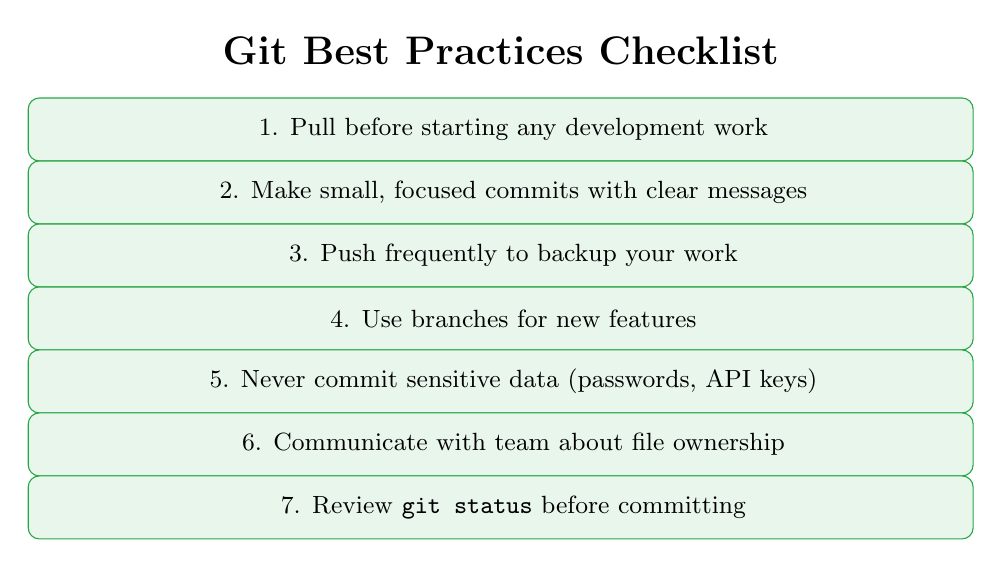
\begin{tikzpicture}[
    node distance=0.5cm,
    practice/.style={rectangle, draw=successgreen, fill=successgreen!10, rounded corners, minimum width=12cm, minimum height=0.8cm, align=left, font=\small}
]
    \node[font=\Large\bfseries] at (0, 4) {Git Best Practices Checklist};

    \node[practice] (p1) at (0, 3) {\quad 1. Pull before starting any development work};
    \node[practice] (p2) at (0, 2.2) {\quad 2. Make small, focused commits with clear messages};
    \node[practice] (p3) at (0, 1.4) {\quad 3. Push frequently to backup your work};
    \node[practice] (p4) at (0, 0.6) {\quad 4. Use branches for new features};
    \node[practice] (p5) at (0, -0.2) {\quad 5. Never commit sensitive data (passwords, API keys)};
    \node[practice] (p6) at (0, -1) {\quad 6. Communicate with team about file ownership};
    \node[practice] (p7) at (0, -1.8) {\quad 7. Review \texttt{git status} before committing};
\end{tikzpicture}
\caption{Git Workflow Best Practices}
\label{fig:best-practices}
\end{figure}

\begin{warning}
Never push anything secret to the remote repository: no passwords, personal API keys, student numbers, or anything you wouldn't want to share with the whole Internet. Once pushed, it's in the history forever!
\end{warning}

%============================================================
\section{Git Command Reference}
%============================================================

\begin{table}[htbp]
\centering
\begin{tabular}{ll}
\toprule
\textbf{Command} & \textbf{Description} \\
\midrule
\texttt{git init} & Initialize a new repository \\
\texttt{git clone <url>} & Clone a remote repository \\
\texttt{git status} & Check current status \\
\texttt{git add <file>} & Stage changes \\
\texttt{git commit -m "msg"} & Create a commit \\
\texttt{git push} & Push to remote \\
\texttt{git pull} & Pull from remote \\
\texttt{git branch} & List branches \\
\texttt{git checkout <branch>} & Switch branches \\
\texttt{git merge <branch>} & Merge a branch \\
\texttt{git log} & View commit history \\
\texttt{git diff} & View changes \\
\texttt{git stash} & Temporarily hide changes \\
\texttt{git remote -v} & View remotes \\
\bottomrule
\end{tabular}
\caption{Essential Git Commands Reference}
\label{tab:git-commands}
\end{table}

%============================================================
\newpage
\section{Exercises}
%============================================================

\begin{tcolorbox}[colback=warningyellow!10, colframe=warningyellow!80!black, title=\textbf{Submission Requirements}]
Submit exercises to Moodle as a single PDF containing the information from Exercises 7, 15, and 16. Deadline: Five days from today.
\end{tcolorbox}

\subsection{Exercise 1: GitHub Account}
Create a GitHub account at \texttt{github.com} with a professional, CV-appropriate username.

\subsection{Exercise 2: Install Git}
Install Git on your computer following the installation instructions for your operating system.

\subsection{Exercise 3: Configure Git}
Configure Git with your name and email using the commands shown in Section 3.2.

\subsection{Exercise 4: Create Commits}
Create a project with:
\begin{itemize}
    \item \texttt{story.txt} (a lengthy text file)
    \item \texttt{shopping\_list.txt} (multiple rows)
    \item \texttt{school/} folder with \texttt{school\_file.txt}
\end{itemize}
Create three commits (one per item) with descriptive messages. Verify with \texttt{git log}.

\subsection{Exercise 5: Staging and Diff}
\begin{enumerate}
    \item Remove staged changes back to modified state
    \item Add items to shopping list
    \item Inspect changes with \texttt{git diff}
    \item Stage changes without committing
    \item Unstage changes
    \item Remove changes entirely so file reverts
\end{enumerate}

\subsection{Exercise 6: Credential Storage}
Configure Git credential helper for your operating system.

\subsection{Exercise 7: GitHub Repository}
Create a public GitHub repository for your project and add it as a remote. Submit the repository link to Moodle.

\subsection{Exercise 8: Push Commits}
Push your commits to the remote repository. Verify all changes are visible on GitHub.

\subsection{Exercise 9: Pull and Sync}
Create a file via GitHub's web interface, then fetch the changes to your local repository.

\subsection{Exercise 10: Stashing}
\begin{enumerate}
    \item Make changes to a tracked file
    \item Stash the changes
    \item Edit a file via GitHub and commit
    \item Edit the same file locally
    \item Use stash to fetch changes
    \item Push all changes to GitHub
\end{enumerate}

\subsection{Exercise 11: Non-Conflicting Merge}
Create two non-conflicting commits (one remote, one local) and merge them using \texttt{git pull}.

\subsection{Exercise 12: Resolve Conflicts}
Intentionally create a merge conflict and resolve it manually. Push the resolved result to GitHub.

\subsection{Exercise 13: History Exploration}
\begin{enumerate}
    \item Create \texttt{secret.txt} with content and commit
    \item Delete \texttt{secret.txt} and commit the deletion
    \item Push to GitHub
    \item Find the secret using commit history (both GitHub and command line)
\end{enumerate}

\subsection{Exercise 14: Clone Repository}
Clone your repository to a different folder, make changes, and push them back.

\subsection{Exercise 15: Team Formation}
Meet your team members and document:
\begin{itemize}
    \item Team member names and GitHub usernames
    \item Team name
    \item Team strengths and weaknesses
    \item Communication platform choice
\end{itemize}

\subsection{Exercise 16: Project Repository Setup}
\begin{enumerate}
    \item Create a GitHub organization
    \item Create a public repository in the organization
    \item Initialize a Spring Boot project with required dependencies
    \item Push to GitHub
    \item Have all team members clone and verify
\end{enumerate}

\subsection{Exercise 17: README Creation}
Create a comprehensive \texttt{README.md} with:
\begin{itemize}
    \item Project title as heading
    \item Project description
    \item Team members with GitHub profile links
\end{itemize}

%============================================================
\vspace{1cm}
\hrule
\vspace{0.3cm}
\begin{center}
\small
\textit{This document is licensed under Creative Commons BY-NC-SA 4.0}
\end{center}

\end{document}
